\section*{Problem 5}
Find the Fourier series for the following signal. 

\begin{figure}[H]
\caption*{}
\centering
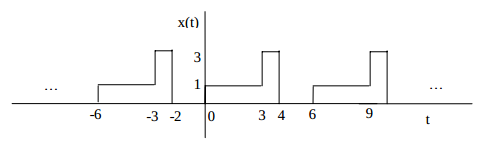
\includegraphics[width=0.7\textwidth]{figs/c1p5.png}
\label{fig:c1p5}
\end{figure} 

Also, sketch the approximation 
if a large number of terms are kept in the series (say N=30).

\subsection*{Solution}

The period of the shown signal is $T=6$ and therefore 
$\omega_0 = \frac{2 \pi}{T} =  \frac{\pi}{3}$.

Taking the derivative of the function we get:
\begin{figure}[H]
\caption{Derivative $\dot{x}$}
\centering
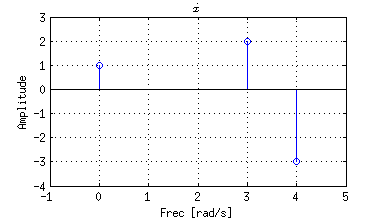
\includegraphics[width=0.6\textwidth]{figs/c1p5a.png}
\label{fig:c1p5a}
\end{figure} 

In the range $[-1, 5]$ we have:

\begin{equation*}
\dot{x}(t) = \delta(t) + 2 \delta(t-3) -3 \delta(t-4)
\end{equation*} 

Applying (\ref{eq:c12}) we have:

\begin{equation*}
\begin{aligned}
j n \omega_0 X_n &= \frac{1}{T} \displaystyle\int_{- T/2}^{T/2}
	[\delta(t) + 2 \delta(t-3) -3 \delta(t-4)]  e^{-j n \omega_0 t} \; dt \\
&=\frac{1}{6} [1 + 2 e^{-2 j n \omega_0} - 3 e^{-4 n j \omega_0}] \\
&=\frac{1}{6} [1 + 2 (-1)^n - 3e^{-\frac{4}{3} j n \pi} ] \\
X_n &= \frac{1}{2 j n \pi}[1 + 2 (-1)^n - 3e^{-\frac{4}{3} j n \pi} ]
\end{aligned}
\end{equation*} 

where 
\begin{equation*}
X_0 = \frac{1}{6} \int_{-1}^{3} x(t) \; dt = 1
\end{equation*} 

The plot for approximating the function using its Fourier coefficients is:

\zcodemat{sources/fapprox5.m}{Approximation of x(t) with Fourier coefficients}

\begin{figure}[H]
\caption{Approximation of x(t) by Xn}
\centering
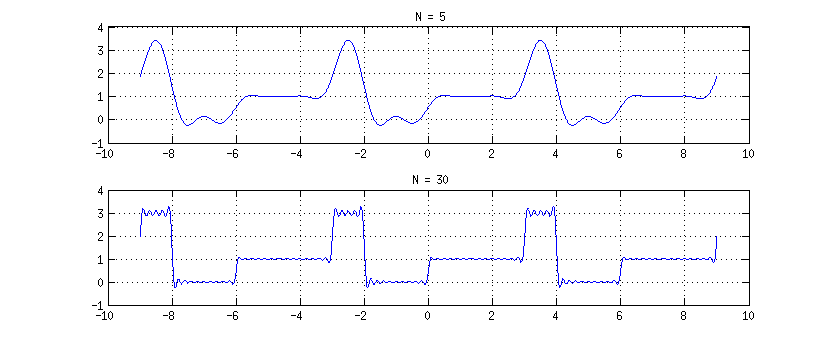
\includegraphics[width=1.0\textwidth]{figs/c1p5b.png}
\label{fig:c1p1c}
\end{figure} 
